\documentclass[../main.tex]{subfiles}
\begin{document}
\chapter{Permutations}
\section{Introduction to Permutations}
Recall that a permutation of a set $X$ is a bijection from $X \to X$ and that $\Sym(X)$ is the group of all such permutations.
\begin{example}
  \label{permutationExample}
  $X = \{1, 2, 3\}$, $\Sym X \cong S_3$
  \begin{center}
  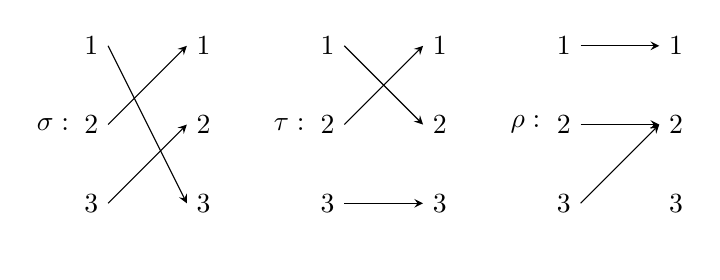
\begin{tikzpicture}[>=stealth]
    \node at (-0.7, 0) {$\sigma:$};
    \draw[->] (0, 1) node[left] {1} -- (1, -1) node[right] {3};
    \draw[->] (0, 0) node[left] {2} -- (1, 1) node[right] {1};
    \draw[->] (0, -1) node[left] {3} -- (1, 0) node[right] {2};
    \node at (0.5, -1.5) {\tick};
    \begin{scope}[xshift=3cm]
      \node at (-0.7, 0) {$\tau:$};
      \draw[->] (0, 1) node[left] {1} -- (1, 0) node[right] {2};
      \draw[->] (0, 0) node[left] {2} -- (1, 1) node[right] {1};
      \draw[->] (0, -1) node[left] {3} -- (1, -1) node[right] {3};

      \node at (0.5, -1.5) {\tick};
    \end{scope}
    \begin{scope}[xshift=6cm]
      \node at (-0.7, 0) {$\rho:$};
      \draw[->] (0, 1) node[left] {1} -- (1, 1) node[right] {1};
      \draw[->] (0, 0) node[left] {2} -- (1, 0) node[right] {2};
      \draw[->] (0, -1) node[left] {3} -- (1, 0);
      \node[right] at (1, -1) {3};
      \node at (0.5, -1.5) {\cross};
    \end{scope}
  \end{tikzpicture}
  \end{center}
  Here, $\sigma$ and $\tau$ are permutations as they are bijective, however, $\rho$ is not as it is not a bijection.

  We can compute composition of permutations using diagrams:
  \begin{center}
  \begin{tikzpicture}
    \node at (0.75, 1.5) {$\sigma$};
    \draw[|->] (0, 1) node[left] {1} -- (1.5, 1) node[right] {3};
    \draw[|->] (0, 0) node[left] {2} -- (1.5, 0) node[right] {1};
    \draw[|->] (0, -1) node[left] {3} -- (1.5, -1) node[right] {2};

    \begin{scope}[xshift=2cm]
      \node at (0.75, 1.5) {$\tau$};
      \draw[|->] (0, 1) -- (1.5, 1) node[right] {3};
      \draw[|->] (0, 0) -- (1.5, 0) node[right] {2};
      \draw[|->] (0, -1) -- (1.5, -1) node[right] {1};
    \end{scope}
  \end{tikzpicture}
  \end{center}
  Because we applied $\sigma$ first and then $\tau$, we write $\tau \sigma$ as it is a composition of functions.
  Drawing diagrams like this is quite cumbersome so we will introduce notation to simplify this.
\end{example}
\subsection{Cycles}
\begin{definition}
  Any list of $k$ \textbf{distinct} elements $a_1, \ldots, a_k \in \{1, \ldots, n\}$ determines a \textit{$k$-cycle}.
  \[
    \sigma = \cycle{a_1 a_2 {\cdots} a_n}
  \]
  as follows:
  \[
    \sigma(b) = \begin{cases}
    a_{i + 1} & \text{ if }b = a_i,\ i < k \\
    a_1 & \text{ if }b = a_k \\
    b & \text{ otherwise}
    \end{cases}
  \]
\end{definition}
\begin{example}
  For the permutations as in \cref{permutationExample}
  \[
    \sigma = \cycle{1 3 2} = \cycle{3 2 1} \text{ and } \tau = \cycle{1 2}
  \]
\end{example}
With practice, you can get proficient at multiplying cycles.
The most important thing to ensure that you \textbf{start from the right}.
\begin{example}
  Using the same permutations again:
  \[
    \tau \sigma = \cycle{1 2}\cycle{1 3 2} = \cycle{1 3}
  \]
  \begin{itemize}
    \item We start by writing 1.
    \item Now check where 1 goes.
      In the first cycle, $1 \mapsto 3$.
      In the second cycle 3 is unchanged.
      So we write 3.
    \item Now we check where 3 goes.
      In the first cycle $3 \mapsto 2$.
      In the second cycle $2 \mapsto 1$.
      We have already written 1 so we are done.
  \end{itemize}
  A more difficult example:
  \[
    \cycle{1 4 3 2}\cycle{2 4 3} = \cycle{1 4 2 3}
  \]
  \begin{itemize}
    \item We start by writing 1.
    \item Now check where 1 goes.
      In the first cycle 1 is unchanged.
      In the second cycle $1 \to 4$.
      So we write 4.
    \item Now check where 4 goes.
      In the first cycle $4 \mapsto 3$.
      In the second cycle $3 \mapsto 2$.
      So we write 2.
    \item Now check where 2 goes.
      In the first cycle $2 \mapsto 4$.
      In the second cycle $4 \mapsto 3$.
      So we write $3.$
    \item Now we check where 3 goes.
      In the first cycle $3 \mapsto 2$.
      In the second cycle $2 \mapsto 1$
      We have already written 1 so we are done.
  \end{itemize}
\end{example}
\begin{remark} Cyclically permuting elements in a cycle does not change the cycle.

  That is:
  \[
    \cycle{a_1 a_2 a_3 {\cdots} a_k} = \cycle{a_2 a_3 {\cdots} a_k a_1} = \cycle{a_3 {\cdots} a_k a_1 a_2}
  \]
  and so on.
\end{remark}
\begin{definition}[Disjoint Cycles]
  Cycles $\cycle{a_1 {\cdots} a_k}$ and $\cycle{b_1 {\cdots} b_k}$ are \textit{disjoint} if $a_i \neq b_j$ for all $i, j$.
\end{definition}
\begin{remark}[Warning]
  In general, cycles \textbf{do not commute}, however disjoint cycles always \textbf{commute}.
\end{remark}
\begin{theorem}[Disjoint Cycles]
  Every $\sigma \in S_n$, can be written as a product of disjoint cycles.

  This expression is unique, up to:
  \begin{itemize}
    \item Shifting elements within a cycle.
    \item Reordering the cycles (as they commute).
  \end{itemize}
\end{theorem}
\begin{proof}
  The action of the subgroup $\langle \sigma \rangle$ on $X = \{1, \ldots, n\}$ partitions $X$ into orbits:
  \[
    X = \langle \sigma \rangle i_1 \cup \langle \sigma \rangle i_2 \cup \cdots \cup \langle \sigma \rangle i_k
  \]
  \textbf{Existence}\par
  Let $n_j = |\langle \sigma \rangle i_j|$.
  We see that:
  \[
    \cycle{i_1 \sigma(i_1) {\cdots} \sigma^{n_1 - 1}(i_1)} \cdots \cycle{i_k \sigma(i_k) {\cdots} \sigma^{n_k - 1}(i_k)}
  \]
  which proves existence.

  \textbf{Uniqueness}\par
  For uniqueness, note that the only choices we made were the orbit representatives $\{i_j\}$ and the indexing function $j \mapsto i_j$.

  Charging orbit representatives simply shifts the elements of a particular cycle as it just starts them at a different element.
  Whereas, changing the indexing permutes the cycles which is possible as the orbits, and therefore the cycles, are disjoint.
\end{proof}
\begin{example}
  When we carry out a multiplication, we naturally write the result as a product of disjoint cycles.
  For example:
  \[
    \cycle{1 2}\cycle{3 4}\cycle{5 6}\cycle{1 2 3 4 5 6} = \cycle{1}\cycle{2 4 6}\cycle{3}\cycle{5} \\
  \]
  In this case, because the 1-cycles do nothing, this happens to just be a single cycle $\cycle{2 4 6}$.
\end{example}
\begin{definition}
  If
  \[
    \sigma = \cycle{a^{1}_{1} {\cdots} a^{1}_{k_1}} \cdots \cycle{a^{l}_{1} {\cdots} a^{l}_{k_l}}
  \]
  is a product of disjoint cycles then $\sigma$ is called a $(k_1, \ldots, k_l)$\textit{-cycle}.
\end{definition}
The set of numbers $\{k_1, \ldots, k_l\}$ is then called the \textit{cycle type} of $\sigma$.
We often omit singletons so a $(3, 2, 1)$-cycle is also referred to as a $(3, 2)$-cycle.
\begin{remark}
  If $\sigma$ is a $k$-cycle, then $|\sigma| = k$.
  More generally, if $\sigma$ is a $(k_1, \ldots, k_l)$-cycle then:
  \[
    |\sigma| = \lcm\{k_1, \ldots, k_l\}
  \]
  as we want the smallest such $n$ so that all the cycles are trivial at the same time.
\end{remark}
\section{Transpositions}
\subsection{Generating \texorpdfstring{$S_n$}{Symmetric Groups}}
\begin{definition}[Transposition]
  A 2-cycle is also called a \textit{transposition} as it transposes two elements.
\end{definition}
\begin{theorem}[Transpositions Generate]
  The set of transpositions generates $S_n$ for any finite $n$.
\end{theorem}
\begin{proof}
  \induction
  {$n = 2$}{
    $S_2 = \{e, \cycle{1 2}\}$
    and the result is obvious \tick
  }
  {$n = k - 1$}{
    So $S_{k - 1}$ is generated by transpositions.
  }
  {$n = k$}{
    Let $\sigma \in S_k$.
    \begin{proofcases}
      \begin{case}{$\sigma(k) = k$}
        Then $\sigma \in S_{k - 1} \leq S_k$ and so:
        \[
          \sigma = \tau_1 \cdots \tau_j
        \]
        for some $j$ and transpositions $\tau_1, \ldots, \tau_j$.
      \end{case}
      \begin{case}{Otherwise}
        Let $\tau = \cycle{k \sigma(k)}$, then:
        \[
          \tau \sigma(k) = \tau(\sigma(k)) = k
        \]
        so $\tau \sigma \in S_{k - 1} \leq S_k$.
        Similarly to above:
        \begin{align*}
          &\tau \sigma = \tau_1 \cdots \tau_j \\
          \implies& \sigma = \tau \tau_1 \cdots \tau_j \text{ (as $\tau^2 = \tau$)}
        \end{align*}
      \end{case}
    \end{proofcases}
    In either case, we can write any $\sigma \in S_k$ as a product of transpositions.
  }
\end{proof}
\begin{definition}[Adjacent Transposition]
  A transposition of the form $\cycle{i {i + 1}}$  is called an \textit{adjacent transposition}.
\end{definition}
\begin{lemma}[Products of Adjacent Transpositions]
  \label{adjacentLemma}
  Any transposition $\cycle{i j}$ can be written as a product of an \textbf{odd} number of adjacent transpositions.
\end{lemma}
\begin{proof}
  WLOG, assume $j > i$ as we can just reorder the transposition.
  \induction
  {$j = i + 1$}{
    Then $\cycle{i j} = \cycle{i {i + 1}}$ which is an adjacent transposition.
  }
  {$j = i + k$}{}
  {$j = i + k + 1$}{
    For $j > i  + 1$, we can write:
    \[
      \cycle{i j} = \underbrace{\cycle{{j - 1} j}}_{\text{adjacent}}\cycle{i {j - 1}}\underbrace{\cycle{{j - 1} j}}_{\text{adjacent}}
    \]
    $j - 1 = i + k$ so, by the induction hypothesis, $\cycle{i {j - 1}}$ can be written as a product of an odd number of adjacent transpositions.
    Therefore $\cycle{i j}$ can be written as a product of adjacent transpositions.
  }
\end{proof}
In particular,we see that $S_n$ is generated by \textbf{adjacent} transpositions.
This discussion leads to a notion of \textit{parity} for permutations.
\subsection{Parity}
We first need to introduce the concept of an \textit{inversion}:
\begin{definition}
  A pair $\{i, j\} \subseteq \{1, \ldots, n\}$ is called an \textit{inversion} of a permutation $\sigma$ if $i < j$ but $\sigma(i) > \sigma(j)$
\end{definition}
\begin{lemma}
  \label{inversionsMod2}
  For any $\sigma = \tau_1 \cdots \tau_k$, $k \equiv \text{\#(inversions of $\sigma$)} \pmod{2}$
\end{lemma}
\begin{proof}
  \induction
  {$k = 0$}{
    So $\sigma = e$ which has no inversions so $k = 0 = \text{\#(inversions of $e$)}$
  }
  {$k -1$}{}
  {$k$}{
    Let:
    \[
      \sigma = \underbrace{\tau_1}_{\tau} \underbrace{\tau_2 \cdots \tau_k}_{\sigma'} = \tau\sigma'
    \]
    where $\tau$ is an adjacent transposition, so we can write $\tau = \cycle{l {l + 1}}$ for some $l$, and $\sigma'$ is the product of $k - 1$ transpositions.

    Now consider which pairs $\{i, j\}$ could be an inversion of $\sigma'$ but not of $\sigma$ and vice versa?

    The only such pairs are those where $\sigma$ sends to either $l$ or $l + 1$.
    So the only such pair is $\{i, j\}$ such that $\sigma(i) = l$ and $\sigma(j) = l + 1$.
    For this pair, we have:
    \[
      \sigma'(i) = l < l + 1 = \sigma'(j)
    \]
    but
    \[
      \sigma(i) = l + 1 > l = \sigma(j)
    \]
    Therefore, if $i < j$, then $\{i, j\}$ is an inversion for $\sigma$ but not for $\sigma'$.
    Whilst if $i > j$, then $\{i, j\}$ is an inversion for $\sigma'$ but not for $\sigma$.
    In either case, $\text{\#(inversions of $\sigma$)} = \text{\#(inversions of $\sigma'$)} \pm 1$.

    By the induction hypothesis, $k - 1 \equiv \text{\#(inversions of $\sigma'$)} \pmod{2}$ so
    \[
      \text{\#(inversions of $\sigma$)} \equiv k - 1 \pm 1 \equiv k \pmod{ 2}
    \]
    Therefore, $k \equiv \text{\#(inversions of $\sigma$)} \pmod{2}$.
  }
\end{proof}
\begin{lemma}
  \label{evenLemma}
  If $\tau_1, \ldots, \tau_k$ are all transpositions and $\sigma = \tau_1 \cdots \tau_k = e$, then $k$ is even.
\end{lemma}
\begin{proof}
  By \cref{adjacentLemma}, we may assume that all $\tau_i$ are adjacent as any non-adjacent transpositions could be rewritten as a product of an \textbf{odd} number of adjacent transpositions which would not change the parity of $k$ (whether $k$ is odd or even).

  If $\sigma = e$, then $\sigma$ has 0 inversions so by \cref{inversionsMod2}, $k$ is even.
\end{proof}
This enables us to define the \textit{sign homomorphism}.
\begin{theorem}[Sign Homomorphism]
  The map:
  \[
    \sign: S_n \to C_2 = \{\pm 1\},\ \tau_1 \cdots \tau_k \mapsto (-1)^{k}
  \]
  is a well defined homomorphism.
\end{theorem}
\begin{proof}\par
  \textbf{Well Defined -} To see that it is well-defined, suppose $\tau_i$ and $\tau_j'$ are all transpositions such that:
  \[
    \tau_1 \cdots \tau_k = \tau_1' \cdots \tau_l'
  \]
  Then, since all transpositions are self inverse:
  \[
    \tau_k \cdots \tau_1 \tau_1' \cdots \tau_l' = e
  \]
  So $k + l$ is even by \cref{evenLemma}.
  Therefore $k \equiv l \pmod{2}$ so $(-1)^{k} = (-1)^{l}$ as required.

  \textbf{Homomorphism -} To see that it is a homomorphism:
  \[
    \sign(\tau_1 \cdots \tau_k \tau_1' \cdots \tau_l') = (-1)^{k + l} = (-1)^{k}(-1)^{l} = \sign(\tau_1 \cdots \tau_k)\sign(\tau_1' \cdots \tau_l')
  \]
\end{proof}
\begin{definition}[Odd and Even Permutations]
  If $\sign(\sigma) = 1$, then $\sigma$ is called an \textit{even permutation}.
  If $\sign(\sigma) = -1$, then $\sigma$ is called an \textit{odd permutation}
\end{definition}
\begin{definition}[Alternating Group]
  The subgroup:
  \[
    A_n = \ker(\sign) \lhd S_n
  \]
  is called the \textit{alternating group} on $n$ elements.
\end{definition}
So $A_n$ is all the \textbf{even} permutations of $S_n$.
\begin{remark}[Note]
  Since $|\im(\sign)| = 2$ and $|\ker(\sign)| = |A_n|$, by \cref{firstIsomorphismCorollary}, we have:
  \[
    |S_n| = 2|A_n|
  \]
\end{remark}
\begin{example}[From $S_3$ to $A_3$]
  \[
    S_3 = \{e, \cycle{1 2}, \cycle{2 3}, \cycle{3 1}, \cycle{1 2 3}, \cycle{3 2 1}\}
  \]
  All the transpositions are odd as they are just a single transposition.
  For the 3-cycles, we have:
  \[
    \cycle{1 2 3} = \cycle{1 2}\cycle{2 3} \text{ and }\cycle{3 2 1} = \cycle{2 3}\cycle{1 2}
  \]
  so both are even, therefore:
  \[
    A_3 = \{e, \cycle{1 2 3}, \cycle{3 2 1}\} \cong C_3
  \]
\end{example}
\begin{remark}
  The cycle type makes it easy to determine the sign of a permutation.

  In the case of a $k$-cycle, we can write:
  \[
    \cycle{a_1 {\cdots} a_k} = \cycle{a_1 a_k}\cycle{a_1 a_{k - 1}} \cdots \cycle{a_1 a_3}\cycle{a_1 a_2}
  \]
  which has $k - 1$ transpositions.
  So a $k$-cycle is \textbf{even} if and only if $k$ is \textbf{odd}.

  More generally, a $(k_1, \ldots, k_l)$-cycle is \textbf{even} if and only if $\#\{\text{even $k_i$}\}$ is \textbf{even}.
  This is because the full cycle is even if and only if we are multiplying an even number of odd cycles.
\end{remark}
\begin{example}
  $\cycle{1 2}\cycle{3 4}$ but $\cycle{1 2}\cycle{3 4}\cycle{5 6}$ is odd.
\end{example}
We can now apply what we have learnt to investigate conjugacy in $S_n$ and $A_n$.
\section{Conjugacy in \texorpdfstring{$S_n$}{Symmetric Groups}}
Conjugacy in $S_n$ is surprisingly simple.
\begin{theorem}
  Two permutations $\sigma_1, \sigma_2 \in S_n$ have the same cycle type if and only if they are conjugate.
\end{theorem}
\begin{proof}
  \begin{proofdirection}{Assume $\sigma_1$ and $\sigma_2$ have the same cycle type}
    So $\sigma_1$ and $\sigma_2$ are both $(l_1, \ldots, l_k)$-cycles.
    We can write:
    \begin{align*}
      \sigma_1 &= \cycle{a^{1}_{1} {\cdots} a^1_{l_1}} \cdots \cycle{a^{k}_{1} {\cdots} a^{k}_{l_k}} \\
      \sigma_2 &= \cycle{b^{1}_{1} {\cdots} b^{1}_{l_1}} \cdots \cycle{b^{k}_{l} {\cdots} b^{k}_{l_k}}
    \end{align*}
    So for some $a^{i}_{j}$, we have:
    \[
      \sigma_1(a^{i}_{j}) = a^{i}_{(j\,+_{l_i} 1)}
    \]
    where $j +_{l_i} 1$ denotes $j + 1$ evaluated mod $l_i$, accounting for when the cycle loops back to the start.
    Similarly for $\sigma_2$:
    \[
      \sigma_2(b^{i}_{j}) = b^{i}_{(j\,+_{l_i} 1)}
    \]
    Since $\sigma_1, \sigma_2 \in S_n$, we can define a permutation $\tau$ of $\{1, \ldots, n\} = \{a^{i}_{j}\} = \{b^{i}_{j}\}$ such that:
    \[
      \tau(a^{i}_{j}) = b^{i}_{j}
    \]
    If we compute $\tau \sigma_1 \tau^{-1}(b^{i}_{j})$, we see that:
    \begin{align*}
      \tau \sigma_1 \tau^{-1}(b^{i}_{j}) &= \tau\sigma_1(a^{i}_{j}) \\
                                         &= \tau\left(a^{i}_{(j\,+_{l_i} 1)}\right) \\
                                         &= b^{i}_{(j\,+_{l_i} 1)} \\
                                         &= \sigma_2 (b^{i}_{j})
    \end{align*}
    Therefore, $\tau\sigma_1\tau^{-1} = \sigma_2$ so they are conjugate, as required.
  \end{proofdirection}
  \begin{proofdirection}{Assume $\sigma_1$ and $\sigma_2$ are conjugate}
    Suppose $\sigma_2 = \tau\sigma_1 \tau^{-1}$,
    The above argument shows that if:
    \[
      \sigma_1 = \cycle{a^{1}_{1} {\cdots} a^1_{l_1}} \cdots \cycle{a^{k}_{1} {\cdots} a^{k}_{l_k}} \\
    \]
    then:
    \[
      \sigma_2 = \cycle{b^{1}_{1} {\cdots} b^{1}_{l_1}} \cdots \cycle{b^{k}_{l} {\cdots} b^{k}_{l_k}}
    \]
    where $b^{i}_{j} = \tau(a^{i}_{j})$ for all $1 \leq i \leq k$ and $i \leq j \leq l$.
    Therefore, $\sigma_1$ and $\sigma_2$ are both $(l_1, \ldots, l_k)$-cycles.
  \end{proofdirection}
\end{proof}
This makes it easy to count conjugacy classes in $S_n$.
\begin{example}[Conjugacy Classes of $S_3$]
  The elements of $S_3$ are:
  \[
    S_3 = \{e, \cycle{1 2}, \cycle{2 3}, \cycle{3 1}, \cycle{1 2 3}, \cycle{3 2 1}\}
  \]
  Suppose we want to count the sizes of each conjugacy class of $S_3$.
  We now know that conjugate elements share the same cycle type so we can use this to compute the sizes of the conjugacy classes.

  For example, to find $|\ccl_{S_3}\cycle{1 2}|$, consider constructing a 2-cycle.
  This involves picking 2 numbers from 3 numbers so there is exactly $\binom{3}{2} = 3$ ways of doing this so $|\ccl_{S_3}\cycle{1 2}| = 3$.

  To find $|\ccl_{S_3}\cycle{1 2 3}|$, consider constructing a 3-cycle.
  There are 3 options for the first element, 2 for the second element and then 1 for the third element so $|\ccl_{S_3} = 2 \cdot 1 =2|$
\end{example}
\begin{example}[A Conjugacy Class in $S_4$]
  Suppose we want to compute the size of the conjugacy class of $(2, 2)$-cycles in $S_4$.
  To construct such an element, we can choose a transposition, and then multiply it by the only possible other transposition.
  There are $\binom{4}{2}$ transpositions but since the order of the two transpositions does not matter we need to half this, yielding:
  \[
    |\ccl_{S_4}(\cycle{1 2}\cycle{3 4})| = \frac{1}{2}\binom{4}{2} = 3
  \]
\end{example}
Recall from \cref{conjugationSec} that under the conjugation action, the centraliser of an element is its stabiliser and the conjugacy class of an element is its orbit.
We can then use Orbit-Stabiliser (\cref{orbitStabiliser}) to see that:
\[
  |C_{S_n}(\gamma)| = \frac{|S_n|}{|\ccl_{S_n}(\gamma)|} = \frac{n!}{|\ccl_{S_n}(\gamma)|}
\]
Since we can count the sizes of conjugacy classes, it is also easy to count the sizes of centralisers.
\begin{example}[Counting a Centraliser]
  Consider the element $\cycle{1 2}\cycle{3 4} \in S_4$.
  \[
    |C_{S_4}(\cycle{1 2}\cycle{3 4})| = \frac{4!}{|\ccl_{S_4}(\cycle{1 2}\cycle{3 4})|} = \frac{24}{3} = 8
  \]
  Since the centraliser of an element can be thought of as the set of element that commute with it, we can simply list elements that commute with it until we have found 8.

  \begin{enumerate}
    \item $e$ always commutes
    \item $\cycle{1 2}\cycle{3 4}$ commutes with itself
    \item $\cycle{1 2}$ commutes as it is disjoint from $\cycle{3 4}$.
    \item $\cycle{3 4}$ commutes as above.
    \item $\cycle{1 3}\cycle{2 4}$ commutes as it just swaps the two transpositions.
    \item $\cycle{1 4}\cycle{2 3}$ commutes as above.
    \item $\cycle{1 4 2 3}$ commutes as it squares to $\cycle{1 2}\cycle{3 4}$. If we have $\sigma^2 = \rho$, then $\sigma \rho = \sigma \sigma^2 = \sigma^2 \sigma = \rho \sigma$ so it commutes.
    \item $\cycle{1 3 2 4}$ commutes as above.
  \end{enumerate}
  We have listed 8, so we know have found the entire centraliser.
\end{example}
\begin{example}[Conjugacy Classes of $S_4$]
  \label{conjugacyS4}
  We can list all of the conjugacy classes in $S_4$.
  \begin{center}
  \renewcommand\arraystretch{1.5}
  \begin{tabular}{c|c|c|>{\small}m{5cm}}
  Typical Element -- $\gamma$ & $|\ccl_{S_4}(\gamma)|$ & $|C_{S_4}(\gamma)|$ & Comment\\
  \hline
  $e$ & 1 & 24 & -- \\
  $\cycle{1 2}$ & $\binom{4}{2} = 6$ & 4 & Covered previously \\
  $\cycle{1 2}\cycle{3 4}$ & $\frac{1}{2}\binom{4}{2} = 3$ & 8 & Covered previously \\
  $\cycle{1 2 3}$ & $2 \binom{4}{3} = 8$ & 3 & $\binom{4}{3}$ to pick, then two orderings by reversing items \\
  $\cycle{1 2 3 4}$ & $3! = 6$ & 4 & Cycle can always start with 1, then $3!$ for remaining items \\
  \end{tabular}
  \end{center}
  The sum of the sizes of the conjugacy classes is 24, the order of the group, which is expected as each element is in exactly one conjugacy class.
\end{example}
\section{Conjugacy in \texorpdfstring{$A_n$}{Alternating Groups}}
Counting conjugacy classes in $A_n$ can be done similarly to as in $S_n$ but requires some additional cases.
\begin{lemma}[Conjuacy Classes in $A_n$]
  \label{conjugacyAn}
  Let $\gamma \in A_n \lhd S_n$.
  \begin{enumerate}
    \item If some odd element of $S_n$ (which will not be in $A_n$) commutes with $\gamma$, then:
      \[
        \ccl_{A_n}(\gamma) = \ccl_{S_n}(\gamma)
      \]
    \item If every element of $S_n$ that commutes with $\gamma$ is even, that is, $C_{S_n}(\gamma) \leq A_n$, then $\ccl_{S_n}(\gamma)$ splits into two as follows:
      \[
        \ccl_{S_n}(\gamma) = \ccl_{A_n}(\gamma) \cup \ccl_{A_n}(\tau \gamma \tau^{-1})
      \]
      where $\tau$ is some odd element of $S_n$ (e.g. a transposition).
  \end{enumerate}
\end{lemma}
\begin{proof}
  Orbit-Stabiliser gives:
  \begin{align*}
    |S_n| &= |\ccl_{S_n}(\gamma)||C_{S_n}(\gamma)| \\
    |A_n| &= |\ccl_{A_n}(\gamma)||C_{A_n}(\gamma)|
  \end{align*}
  Since $|S_n| = 2|A_n|$, this gives:
  \begin{equation}
    \label{conjugacyStar}
    |\ccl_{S_n}(\gamma)| = 2 \left[\frac{|C_{A_n}(\gamma)||\ccl_{A_n}(\gamma)|}{|C_{S_n(\gamma)}|}\right] \tag{\textasteriskcentered}
  \end{equation}
  We also have that:
  \[
    C_{A_n}(\gamma) = \ker(\sign |_{C_{S_n}(\gamma)}: C_{S_n(\gamma)} \to C_2)
  \]
  that is, $C_{A_n}(\gamma)$ is the kernel of the sign function restricted to $C_{S_n}(\gamma)$.
  The image has either size 1, if the elements of $C_{S_n}(\gamma)$ are all even, or 2, if the some of the elements are odd.
  Then, by the isomorphism theorem (\cref{isomorphismTheorem}),
  \[
    |C_{S_n}(\gamma) : C_{A_n}(\gamma)| = 1 \text{ or }2
  \]
  \begin{enumerate}
    \item If there is an odd element of $S_n$ that commutes with $\gamma$, then:
      \[
        |C_{S_n}(\gamma) : C_{A_n}(\gamma)| = 2
      \]
      Using Lagrange and \cref{conjugacyStar}, we then have:
      \[
        |\ccl_{S_n}(\gamma)| = \frac{2|C_{A_n}(\gamma)|}{2|C_{A_n}(\gamma)|}|\ccl_{A_n}(\gamma)| = |\ccl_{A_n}(\gamma)|
      \]
      So no elements of the conjugacy class are lost when we restrict to only even permutations, thus, $\ccl_{S_n}(\gamma) = \ccl_{A_n}(\gamma)$, as required.
    \item The hypothesis means that:
      \[
        C_{S_n}(\gamma) = C_{A_n}(\gamma)
      \]
      as no elements are lost when we restrict from $A_n$ to $S_n$
      so using \cref{conjugacyStar}, we then have:
      \[
        |\ccl_{S_n}(\gamma)| = 2 |\ccl_{A_n}(\gamma)|
      \]
      So $\ccl_{A_n}(\gamma)$ is half as big.

      Now consider an odd permutation $\tau \in S_n$.
      Note that $\tau \gamma \tau^{-1} \in \ccl_{S_n}(\gamma)$.
      Suppose that $\tau \gamma \tau^{-1} \in \ccl_{A_n}(\gamma)$ then:
      \[
        \tau\gamma\tau^{-1} = \alpha \gamma \alpha^{-1}
      \]
      for some $\alpha \in A_n$.
      But then:
      \[
        (\tau \alpha)\gamma(\tau \alpha)^{-1} = \gamma \iff (\tau \alpha)\gamma = \gamma(\tau\alpha)
      \]
      so $\tau \alpha \in C_{S_n}(\gamma) = C_{A_n}(\gamma)$.
      But $\tau \alpha$ is odd, so we have arrived at a contraction.
      Hence $\tau \gamma \tau^{-1} \notin \ccl_{A_n}(\gamma)$.
      So it follows that $C_{S_n}(\gamma)$ was split into $\ccl_{A_n}(\gamma)$ and $\ccl_{A_n}(\tau \gamma \tau^{-1})$
  \end{enumerate}
\end{proof}
This makes it possible to determine conjugacy classes in $A_n$.
\begin{example}[Conjuacy Classes in $A_4$]
  The even elements of $S_4$ are $e$, $(2, 2)$-cycles, and 3-cycles.

Since there is an odd number of $(2, 2)$-cycles, we cannot split the conjugacy class in half, so $\ccl(\cycle{1 2}\cycle{3 4})$ remains intact in $A_4$.

  For a 3-cycle, $\sigma = \cycle{1 2 3}$:
  \[
    |C_{S_4} \cycle{1 2 3}| = 3
  \]
  The subgroup generated by $\cycle{1 2 3}$ has three elements, all of which certainly commute with $\cycle{1 2 3}$ so:
  \[
    C_{S_4}(\cycle{1 2 3}) = \langle \cycle{1 2 3} \rangle \leq A_4
  \]
  All of the elements in this subgroup are even by \cref{conjugacyAn}, $\ccl_{S_4}\cycle{1 2 3}$ splits.
  One half is just the even permutations of $\ccl_{S_4}\cycle{1 2 3}$.
  The other half can be obtained by taking the conjugate of $\cycle{1 2 3}$ by any odd permutation, such as $\cycle{1 2}$ to get $\cycle{1 2}\cycle{1 2 3}\cycle{1 2} = \cycle{3 2 1}$, the other half is then $\ccl_{A_4}\cycle{3 2 1}$.

  In summary:
  \begin{center}
  \begin{tabular}{c|c|>{\small}m{5cm}}
    Typical Element ($\gamma$) & $|\ccl_{A_4}(\gamma)|$ & Comment\\
  \hline
  $e$ & 1 & --\\
  $\cycle{1 2}\cycle{3 4}$ & 3 & Does not split \\
  $\cycle{1 2 3}$ & 4 & From \cref{conjugacyS4}, it has order 8 in $S_4$ and splits in half so has order 4\\
  $\cycle{3 2 1}$ & 4 & Other half of $\ccl_{S_4}\cycle{1 2 3}$, that is, $\ccl_{A_4}(\tau \cycle{1 2 3} \tau^{-1})$ for odd $\tau \in S_4$ \\
  \end{tabular}
  \end{center}
  If we sum the sizes of the conjugacy classes we get $12 = \frac{24}{2} = |A_4|$ as expected.
\end{example}
\end{document}
